\documentclass[11pt]{article}
\usepackage{amsmath}
\usepackage{amssymb}
\usepackage[hidelinks]{hyperref}
\usepackage[T1]{fontenc}
\usepackage[a4paper]{geometry}
\geometry{verbose,tmargin=3cm,bmargin=2cm,lmargin=2cm,rmargin=3cm,headheight=2.5cm,headsep=0.5cm}
\usepackage{fancyhdr}
\pagestyle{fancy}
\usepackage{graphicx}
\usepackage{multirow}
\usepackage{setspace}
\onehalfspacing
\usepackage{blindtext}
\usepackage[utf8]{inputenc}
\usepackage{float}
\usepackage{hyperref}
\usepackage[normalem]{ulem}
\usepackage{listings}
\usepackage{xcolor}


\usepackage[lastpage,user]{zref}
\usepackage{fancyhdr}
\pagestyle{fancy}
\cfoot{\thepage\ de \zpageref{LastPage}}

\lstdefinestyle{common}{
  basicstyle=\ttfamily\small,
  keywordstyle=\color{blue},
  commentstyle=\color{gray},
  stringstyle=\color{red},
  numbers=left,
  numberstyle=\tiny\color{gray},
  stepnumber=1,
  numbersep=5pt,
  showstringspaces=false,
  breaklines=true,
  frame=single,
  tabsize=2
}

\lstdefinelanguage{PostgreSQL}{
  sensitive=true,
  morekeywords={
    CREATE, TABLE, VIEW, MATERIALIZED, INDEX, UNIQUE, PRIMARY, FOREIGN, KEY, CONSTRAINT, DROP, ALTER, ADD,
    RENAME, TO, SEQUENCE, OWNED, BY,
    SELECT, INSERT, INTO, VALUES, UPDATE, DELETE, FROM, WHERE, SET, RETURNING,
    ORDER, BY, GROUP, HAVING, LIMIT, OFFSET, DISTINCT,
    JOIN, INNER, LEFT, RIGHT, FULL, OUTER, ON, USING, NATURAL,
    AND, OR, NOT, IS, NULL, TRUE, FALSE, UNKNOWN,
    INTEGER, INT, BIGINT, SMALLINT, SERIAL, BIGSERIAL,
    DECIMAL, NUMERIC, REAL, DOUBLE, PRECISION,
    MONEY, TEXT, VARCHAR, CHAR, CHARACTER, BOOLEAN, DATE, TIME, TIMESTAMP, INTERVAL, BYTEA,
    UUID, JSON, JSONB, XML,
    COUNT, AVG, SUM, MIN, MAX, NOW, CURRENT_DATE, CURRENT_TIME, CURRENT_TIMESTAMP,
    EXTRACT, AGE, CAST, COALESCE, NULLIF,
    AS, IN, ANY, ALL, EXISTS, CASE, WHEN, THEN, ELSE, END, LIKE, ILIKE, SIMILAR, ESCAPE,
    BETWEEN, INHERITS, DEFAULT, WITH, WITHOUT, OIDS, OWNER, GRANT, REVOKE,
    BEGIN, END, DECLARE, EXCEPTION, LOOP, IF, ELSIF, ELSEIF, ELSE, THEN, WHILE, FOR, IN, EXECUTE, PERFORM,
    LANGUAGE, PLPGSQL, RETURNS, FUNCTION, IMMUTABLE, STABLE, VOLATILE, SECURITY, DEFINER, INVOKER
  },
  morecomment=[l]{--},
  morecomment=[s]{/*}{*/},
  morestring=[b]',
  alsoletter={\#},
  moredelim=**[is][\color{orange}]{@}{@}, % For optional emphasis like @text@
}

\def\myPath{databases/2024edition/content/}

\begin{document}
\lhead{
\includegraphics[scale=0.3]{./img/uncuyo-logo.png}}
\rhead{
\includegraphics[scale=0.4]{./img/uncuyo-fing-logo.png}}

\vspace{2cm}

\begin{singlespace}
\begin{center}
\rule{1\columnwidth}{2pt}
\par\end{center}

\begin{center}
{\Large{}LICENCIATURA EN CIENCIAS DE LA COMPUTACIÓN}{\Large\par}
\par\end{center}

\begin{center}
{\Large{}Teoría de Base de Datos}{\Large\par}
\par\end{center}

\begin{center}
\textbf{\large Proyecto Integrador}   \end{center}

\begin{center}
Alumno: Gonzalo Padilla Lumelli
\par\end{center}

\begin{center}
\rule{1\columnwidth}{2pt}    
\end{center}

\vspace{10em}

\begin{center}
\rule{1\columnwidth}{4pt}    
\end{center}

\begin{center}
\Large \textbf{PedidosNow}
\par\end{center}

\begin{center}
\rule{1\columnwidth}{4pt}    
\end{center}

\end{singlespace}

\newpage

\tableofcontents

\newpage

%ETAPA 1

\section{Descripción de la empresa}

PedidosNow es una empresa argentina fundada en 2010 que ofrece un servicio de gestión y seguimiento de pedidos de comida a domicilio. Desde su creación, se ha expandido a más de 20 países en Latinoamérica y cuenta con una base de más de 30 millones de usuarios, más de 15,000 cadenas de restaurantes afiliadas y aproximadamente 300,000 repartidores registrados. La empresa procesa más de 23 millones de pedidos anuales, con ingresos que superan los \$3,500 millones de dólares y una valuación en bolsa de \$35,000 millones de dólares.

El servicio de PedidosNow funciona a través de un sistema de software disponible en sitio web y aplicaciones móviles, que conecta a clientes, restaurantes y repartidores de manera eficiente. Los clientes pueden explorar restaurantes, realizar pedidos, pagar en línea y hacer seguimiento en tiempo real de sus envíos. Los restaurantes pueden registrar sus sucursales, cargar su menú, gestionar pedidos y acceder a estadísticas sobre su desempeño. Los repartidores, por su parte, pueden elegir sus horarios y zonas de trabajo, recibiendo incentivos financieros en función de la demanda.

Para optimizar la logística de entrega, PedidosNow asigna automáticamente cada pedido al repartidor y restaurante más convenientes, minimizando tiempos y costos de envío. Además, el sistema ofrece soporte a clientes, restaurantes y repartidores, garantizando la mejor experiencia posible a través de atención al cliente, gestión de reembolsos y resolución de problemas en los envíos.

La empresa se organiza en diferentes áreas clave: gerencia, tecnología y desarrollo de producto, operaciones y logística, marketing, recursos humanos, finanzas y legal, y atención al cliente. Cada una de estas áreas contribuye al crecimiento y éxito de la plataforma, asegurando una operación eficiente y en constante evolución.

\subsection{Actividades que realiza la empresa}

La actividad principal de la empresa es desarrollar y mantener un sistema de software, donde los clientes pueden realizar pedidos de comida a domicilio en más de 15,000 restaurantes, desde su computadora o dispositivo móvil. También permite a restaurantes registrarse y ofrecer sus productos a través de PedidosNow, y a sus repartidores registrados la capacidad de elegir sus horarios y zonas de trabajo. Para cumplir con esta misión, la empresa actúa como intermediaria entre tres tipos de entidades: clientes, restaurantes y repartidores.

La empresa, además, se encarga de la logística del reparto de los envíos, asignando cada orden realizada, al repartidor y a la sucursal (en caso de una cadena de restaurantes) más convenientes, según sus ubicaciones, horario de trabajo del repartidor, etc. El sistema busca evitar que el tiempo de los repartidores y restaurantes sea desaprovechado, a la vez que intenta minimizar el costo y tiempo de envío. Para ello, ofrece incentivos financieros a los repartidores, a través de comisiones más altas, para que elijan trabajar en las zonas geográficas y horarios con mayor demanda.

La empresa ofrece su servicio a través de un sitio web y aplicaciones móviles para iOS y Android. Tanto clientes, como restaurantes y repartidores, utilizan este sistema de software para interactuar con PedidosNow.

\subsubsection{Actividades relacionadas a los clientes}

Los clientes son los usuarios principales de la aplicación. El sistema cuenta con la capacidad de registrar clientes nuevos, y permite a los clientes ya registrados iniciar sesión. El cliente puede cargar distintas direcciones de envío para sus pedidos.

En la página principal, permite a los clientes explorar los distintos restaurantes que ofrecen sus productos a través de PedidosNow. El cliente puede observar los distintos productos de cada restaurante, sus precios y si hay stock disponible. De cada restaurante, se indican el tiempo estimado de entrega, costo de envío, horarios de atención, y reseñas y puntuaciones realizadas por otros usuarios.

El cliente tiene la posibilidad de agregar productos de un restaurante a su carrito de compras, siempre que el mismo se encuentre abierto y el producto en cuestión se encuentre en stock. Solo puede agregar productos de un mismo restaurante. Si el sistema detecta que el restaurante está muy lejos de la dirección de envío del cliente, le alertará que no podrá realizar la compra a menos que cambie su dirección a la hora de realizar la compra.

Una vez que el cliente ha agregado todos los productos que le interesan comprar al carrito, puede proceder con la compra. Primero debe indicar la dirección de envío, ya sea una cargada anteriormente, o una nueva. Si el restaurante se encuentra demasiado lejos, o no hay repartidores disponibles, no se podrá proceder con la compra. De lo contrario, solicita al usuario el medio de pago a utilizar, y el ingreso de los datos requeridos por el mismo (Nº de tarjeta, código de seguridad, etc.).

Si el pago es exitoso, se envía la orden a la sucursal más ideal para que comience su preparación, y se asigna el repartidor más conveniente para el reparto del pedido.

Una vez realizada la compra, el sistema ofrece al cliente la capacidad de realizar el rastreo y seguimiento de su pedido, indicándose el estado actual del mismo, detalles de la compra y el pago, detalles del repartidor asignado (nombre, ubicación), tiempo estimado de finalización, etc. El cliente no podrá realizar más de un pedido a la vez.

El cliente tiene un breve periodo de tiempo, antes de que el restaurante empiece a preparar la orden, para cancelarla. También puede hacerlo si el tiempo de envío excede por mucho el tiempo estimado al realizar la compra.

Si el envío es imposible de realizar debido a razones de fuerza mayor, se alerta al cliente que el envío fue cancelado y se le realiza un reembolso inmediato.

Por otro lado, si el envío es completado con éxito, el cliente puede dejar una puntuación y reseña del restaurante. También puede ver un historial de sus pedidos realizados anteriormente.

Si el cliente no está conforme con el envío, puede solicitar un reembolso a través de la aplicación.

\subsubsection{Actividades relacionadas a los restaurantes}

Cualquier restaurante habilitado en las ciudades donde opera PedidosNow puede registrarse con la empresa para ofrecer sus productos a través de la app. La carga de un restaurante nuevo no es completamente automática, sino que requiere verificación humana de la autenticidad del mismo y de su habilitación para operar.

Como condición para trabajar con la empresa, deben pagar como comisión cada mes un porcentaje de sus ingresos totales obtenidos a través de PedidosNow.

Las grandes cadenas de restaurantes pueden acceder a contratos más beneficiosos con comisiones más bajas, si cumplen con ciertos volúmenes de venta mínimos, o acuerdan no trabajar con servicios de reparto competidores.

El sistema permite a los dueños de los restaurantes cargar sus sucursales, productos (con sus precios, imágenes, descripción, tiempo de preparación, etc.), niveles de stock, etc.

PedidosNow también ofrece a los restaurantes, estadísticas y analíticas de las ventas realizas, productos más buscados, y otros datos de utilidad para que los restaurantes puedan mejorar su servicios.

Si por alguna razón, se hiciese imposible la realización de una orden, el restaurante puede cancelar el pedido pero deberá pagar una multa a PedidosNow.

\subsubsection{Actividades relacionadas a los repartidores}

La empresa ofrece a cualquier mayor de 18 años con un vehículo apto para reparto y un DNI válido la posibilidad de trabajar como repartidor en su servicio. Los interesados en ser repartidores deben registrarse como tal en la app, subir la documentación requerida, y esperar a ser aprobados por una verificación humana.

Cada repartidor recibe una comisión por cada pedido realizado con éxito.

Permite a los repartidores la capacidad de elegir sus horarios y zonas de trabajo, aunque ofrece de forma dinámica comisiones más altas en los horarios y zonas con más demanda de pedidos.

Durante Asigna a los repartidores los pedidos a realizar, indicándoles las direcciones de partida y llegada, detalles de la orden, y algunos datos del cliente.

Si el repartidor tiene un inconveniente de fuerza mayor al realizar el pedido, puede contactar a soporte a través de la app para que sea cancelado, aunque no cobrará comisión. También puede cancelar el envío actual e incluso su turno de trabajo antes de tiempo, pero además de no cobrar comisión, será penalizado con multas.


\subsection{Estructura de la empresa}

La empresa está organizada en las siguientes áreas:

\begin{itemize}
    \item Gerencia
    
    Consiste de los ejecutivos de alto nivel, incluyendo al CEO, COO, CFO, CTO y CMO. Decide los objetivos y metas de la empresa, toma las decisiones de mayor responsabilidad, y realiza acuerdos de gran envergadura con otras empresas.

    \item Tecnología y Desarrollo del Producto
    
    Encargada principalmente de mantener el software y la infraestructura de la empresa. También está encargada de la ciberseguridad y del análisis de datos.

    \item Operaciones y Logística
    
    Su principal tarea es manejar los acuerdos con los restaurantes. También es responsable de mantener la cantidad adecuada de repartidores disponible y la correcta asignación de los pedidos.

    \item Comercial y Alianzas Estratégicas
    
    Se encarga de atraer y gestionar restaurantes y comercios, negociando condiciones, acuerdos y asegurando buenas relaciones con los socios comerciales.

    \item Marketing
    
    Responsable de las campañas de marketing, SEO, retención de usuarios, promociones, la identidad de la marca, y el uso de redes sociales.

    \item Recursos Humanos
    
    Se encarga de la contratación de personal, pago de sueldos y beneficios.

    \item Finanzas y Legal
    
    Se encarga de llevar la contabilidad de la empresa y cumplir con sus obligaciones financieras y legales.

    \item Atención al Cliente
    
    Provee soporte a clientes, restaurantes y repartidores respecto al uso de la plataforma, reembolsos, problemas con los envíos, etc.
\end{itemize}

\subsection{Organigrama de la empresa}
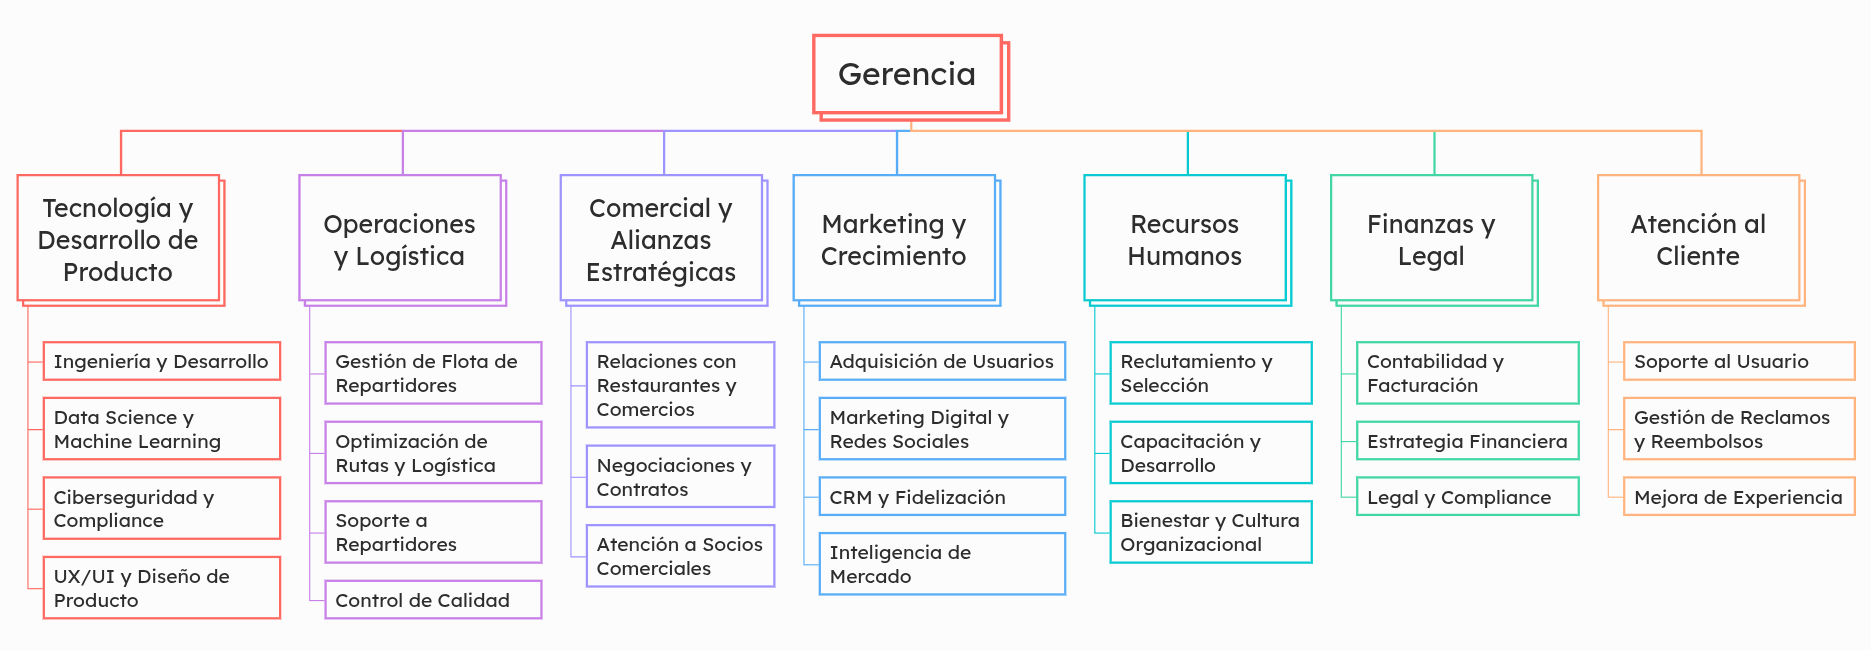
\includegraphics[scale=0.27]{./img/organigrama.png}


%Etapa 2

\section{Descripción del sistema a desarrollar}

\subsection{Motivación para desarrollar el sistema}

\subsection{Descripción de usuarios del sistema}

\subsection{Requisitos funcionales del sistema}

\subsection{Requisitos no funcionales del sistema}

\subsection{Límites y alcances del sistema}


%Etapa 3

\section{Diagrama Entidad Relación de la Base de Datos}

\subsection{Diagrama Entidad Relación (DER)}

\begin{figure}[H]
    \centering
    \includegraphics[width=\linewidth]{./img/der.pdf}
    \caption{Diagrama Entidad Relación del modelo de datos. También puede acceder al mismo en el siguiente link: \url{https://lucid.app/lucidchart/2b762760-f1e0-41fe-a088-a1b024189f9b/edit?invitationId=inv_071c5e9c-b232-40a7-a489-c9ad35b91a7a}}
\end{figure}

\subsection{Descripción del DER}

\textbf{Entidades}
\begin{enumerate}
    \item \textbf{Cliente:} Representa a un cliente registrado en la plataforma. Son los que realizan pedidos a domicilio.
    
    \textbf{Tipo:} Fuerte \\
    \textbf{Clave:} \texttt{id} \\
    \textbf{Atributos:}
    \begin{itemize}
        \item \texttt{id}: Identificador único para cada cliente.
        \item \texttt{email}: Email del cliente.
        \item \texttt{nombre}: Nombre del cliente.
        \item \texttt{fecha\_nacimiento}: Fecha de nacimiento del cliente.
        \item \texttt{fecha\_registro}: Fecha de registro del cliente.
    \end{itemize}

    \item \textbf{Repartidor:} Representa a un repartidor registrado en la plataforma. Realizan los envíos a domicilio.
    
    \textbf{Tipo:} Fuerte \\
    \textbf{Clave:} \texttt{id} \\
    \textbf{Atributos:}
    \begin{itemize}
        \item \texttt{id}: Identificador único para cada repartidor.
        \item \texttt{email}: Email del repartidor.
        \item \texttt{nombre}: Nombre del repartidor.
        \item \texttt{fecha\_nacimiento}: Fecha de nacimiento del repartidor.
        \item \texttt{tipo\_de\_vehículo}: Tipo de vehículo (bicicleta, moto, auto, etc.) del repartidor.
        \item \texttt{patente}: Patente del vehículo (si aplica).
        \item \texttt{fecha\_alta}: Fecha de alta del repartidor.
    \end{itemize}
    
    \item \textbf{Restaurante:} Representa a un restaurante, que puede tener una o más sucursales.
    
    \textbf{Tipo:} Fuerte \\
    \textbf{Clave:} \texttt{id} \\
    \textbf{Atributos:}
    \begin{itemize}
        \item \texttt{id}: Identificador único para cada restaurante.
        \item \texttt{email}: Email de la cuenta del restaurante.
        \item \texttt{nombre\_restaurante}: Nombre del restaurante.
        \item \texttt{domicilio\_legal}: Domicilio legal del restaurante.
        \item \texttt{fecha\_registro}: Fecha de registro del restaurante.
        \item \texttt{url\_logo}: url del logo del restaurante.
    \end{itemize}
    
    \item \textbf{Sucursal:} Representa a una sucursal en particular de un restaurante.
    
    \textbf{Tipo:} Fuerte \\
    \textbf{Clave:} \texttt{id} \\
    \textbf{Atributos:}
    \begin{itemize}
        \item \texttt{id}: Identificador único para cada sucursal.
        \item \texttt{nombre\_sucursal}: Nombre de la sucursal.
        \item \texttt{está\_abierta}: Si está abierta o cerrada.
        \item \texttt{url\_logo}: url del logo de la sucursal.
    \end{itemize}
    
    \item \textbf{Ítem Menú:} Un item del menú ofrecido por alguna sucursal de un restaurante.
    
    \textbf{Tipo:} Fuerte \\
    \textbf{Clave:} \texttt{id} \\
    \textbf{Atributos:}
    \begin{itemize}
        \item \texttt{id}: Identificador único para cada ítem del menú.
        \item \texttt{nombre}: Nombre del ítem del menú.
        \item \texttt{descripción}: Descripción del ítem del menú.
        \item \texttt{url\_imagen}: url de una imagen del ítem del menú.
    \end{itemize}

    \item \textbf{Categoría Ítem Menú:} Categoría a la cuál puede pertenecer un ítem del menú.
    
    \textbf{Tipo:} Fuerte \\
    \textbf{Clave:} \texttt{id} \\
    \textbf{Atributos:}
    \begin{itemize}
        \item \texttt{id}: Identificador único para cada categoría.
        \item \texttt{nombre\_categoría}: Nombre de la categoría.
    \end{itemize}
    
    \item \textbf{Dirección:} La dirección de algún domicilio.
    
    \textbf{Tipo:} Fuerte \\
    \textbf{Clave:} \texttt{id} \\
    \textbf{Atributos:}
    \begin{itemize}
        \item \texttt{id}: Identificador único para cada dirección.
        \item \texttt{provincia}: Provincia.
        \item \texttt{municipio}: Municipio (departamento o partido).
        \item \texttt{localidad}: Localidad.
        \item \texttt{calle}: Calle.
        \item \texttt{número}: Numeración.
        \item \texttt{piso}: Piso.
        \item \texttt{depto}: Departamento.
        \item \texttt{tel}: Teléfono de contacto.
        \item \texttt{observación}: Observación adicional respecto a la dirección.
        \item \texttt{latitud}: Latitud de la dirección.
        \item \texttt{longitud}: Longitud de la dirección.
    \end{itemize}
    
    \item \textbf{Orden:} Representa una order realizada por un cliente a la sucursal de algún restaurante. También funciona como carrito de compras antes de que se realice el pago.
    \textbf{Tipo:} Fuerte \\
    \textbf{Clave:} \texttt{id} \\
    \textbf{Atributos:}
    \begin{itemize}
        \item \texttt{id}: Identificador único para cada orden.
        \item \texttt{estado}: Estado de la orden (en el carrito, en preparación, preparada, en camino, entregada, cancelada).
        \item \texttt{subtotal}: Subtotal de la orden.
        \item \texttt{costo\_envío}: Costo del envío.
        \item \texttt{propina}: Propina para el repartidor.
        \item \texttt{total}: Costo total de la orden.
        \item \texttt{tiempo\_de\_inicio}: Fecha y hora a la que fue encargada la orden.
        \item \texttt{tiempo\_de\_entrega}: Fecha y hora a la que fue entregada la orden.
    \end{itemize}

    \item \textbf{Reseña:} Reseña de una orden, realizada por un cliente.
    
    \textbf{Tipo:} Fuerte \\
    \textbf{Clave:} \texttt{id} \\
    \textbf{Atributos:}
    \begin{itemize}
        \item \texttt{id}: Identificador único para cada reseña.
        \item \texttt{texto\_reseña}: Texto de la reseña.
        \item \texttt{rating}: Rating, de 1 a 5 estrellas.
    \end{itemize}
\end{enumerate}

\textbf{Relaciones}
\begin{enumerate}
    \item \textbf{TIENE DIRECCIÓN (Cliente - Dirección):} Un cliente tiene de cero a muchas direcciones. Una dirección tiene un cliente.

    \textbf{Cardinalidad:} 1:N \\
    \textbf{Participación:} Parcial en Cliente, total en Dirección \\
    \textbf{Roles:} Cliente (tiene dirección en), Dirección (pertenece a) \\
    \textbf{Atributos:}
    \begin{itemize}
        \item \texttt{es\_dirección\_por\_defecto}: Si es la dirección por defecto de un cliente.
    \end{itemize}

    \item \textbf{TIENE SUCURSAL (Restaurante - Sucursal):} Un restaurante tiene una o más sucursales. Una sucursal es de un restaurante.

    \textbf{Cardinalidad:} 1:N \\
    \textbf{Participación:} Total en Restaurante, total en Sucursal \\
    \textbf{Roles:} Restaurante (tiene sucursal), Sucursal (es sucursal de)

    \item \textbf{PROVEE (Sucursal - Ítem Menú):} Una sucursal provee muchos ítems del menú. Un ítem del menú es provisto por una sola sucursal.

    \textbf{Cardinalidad:} 1:N \\
    \textbf{Participación:} Parcial en Sucursal, total en Ítem Menú \\
    \textbf{Roles:} Sucursal (provee), Ítem Menú (es provisto por) \\
    \textbf{Atributos:}
    \begin{itemize}
        \item \texttt{disponible}: Si el ítem del menú se encuentra disponible en esa sucursal.
        \item \texttt{precio\_actual}: Precio actual del ítem del menú en esa sucursal.
    \end{itemize}

    \item \textbf{ES DE TIPO (Ítem Menú - Categoría Ítem Menú):} Un ítem del menú es de un tipo de categoría. Una categoría puede contener de cero a muchos ítems de menú.

    \textbf{Cardinalidad:} 1:N \\
    \textbf{Participación:} Total en Item, parcial en Categoría Ítem Menú \\
    \textbf{Roles:} Ítem Menú (es de tipo), Categoría Ítem Menú (contiene) \\

    \item \textbf{UBICADA EN DIRECCIÓN (Sucursal - Dirección):} Una sucursal se encuentra ubicada en una dirección. En una dirección se encuentra ubicada una o ninguna sucursal.

    \textbf{Cardinalidad:} 1:1 \\
    \textbf{Participación:} Total en Sucursal, parcial en Dirección \\
    \textbf{Roles:} Sucursal (ubicada en), Dirección (contiene una)

    \item \textbf{ENCARGADA POR (Orden - Cliente):} Una orden es encargada por un cliente. Un cliente encarga de cero a muchas órdenes.

    \textbf{Cardinalidad:} 1:N \\
    \textbf{Participación:} Total en Orden, parcial en Cliente \\
    \textbf{Roles:} Orden (encargada por), Cliente (encarga)

    \item \textbf{PREPARADA POR (Orden - Sucursal):} Una orden es preparada por una sucursal. Una sucursal prepara de cero a muchas órdenes.

    \textbf{Cardinalidad:} 1:N \\
    \textbf{Participación:} Total en Orden, parcial en Cliente \\
    \textbf{Roles:} Orden (preparada por), Sucursal (prepara)

    \item \textbf{REPARTIDA POR (Orden - Repartidor):} Una orden es repartida por ningún o un solo repartidor. Un repartidor reparte de cero a muchas órdenes.

    \textbf{Cardinalidad:} 1:N \\
    \textbf{Participación:} Parcial en Orden, parcial en Repartidor \\
    \textbf{Roles:} Orden (repartida por), Repartidor (reparte)

    \item \textbf{DIRIGIDA A (Orden - Dirección):} Una orden está dirigida a una dirección. A una dirección están dirigidas de cero a muchas órdenes.

    \textbf{Cardinalidad:} 1:N \\
    \textbf{Participación:} Total en Orden, parcial en Dirección \\
    \textbf{Roles:} Orden (dirigida a), Dirección (recibe)
    
    \item \textbf{CONTIENE (Orden - Ítem Menú):} Una orden contiene de uno a muchos ítems del menú. Un ítem del menú puede estar contenido en cero o muchas órdenes.

    \textbf{Cardinalidad:} N:M \\
    \textbf{Participación:} Total en Orden, parcial en Ítem Menú \\
    \textbf{Roles:} Orden (contiene), Ítem Menú (contenido en) \\
    \textbf{Atributos:}
    \begin{itemize}
        \item \texttt{disponible}: Si el ítem del menú se encuentra disponible en esa sucursal.
        \item \texttt{precio\_actual}: Precio actual del ítem del menú en esa sucursal.
    \end{itemize}

    \item \textbf{ESCRITA POR (Cliente - Orden - Reseña):} Una reseña referida a una orden, es escrita por un solo cliente. Una reseña escrita por un cliente, se refiere a una sola orden. Una orden realizada por un cliente, puede tener o no una reseña.

    \textbf{Cardinalidad:} 1:1:1 \\
    \textbf{Participación:} Parcial en Cliente, parcial en Orden, total en Reseña \\
    \textbf{Roles:} Una reseña referida a una orden (escrita por) un cliente. Una reseña escrita por un cliente (se refiere a) una orden. Una orden realizada por un cliente, (tiene) una reseña.

    \item \textbf{TIENE RESEÑA (Sucursal - Reseña):} Una sucursal puede tener entre cero y muchas reseñas. Una reseña es acerca de una sola sucursal.

    \textbf{Cardinalidad:} 1:N \\
    \textbf{Participación:} Total en Reseña, parcial en Sucursal \\
    \textbf{Roles:} Sucursal (tiene) reseñas. Reseña (acerca de) Sucursal.
\end{enumerate}

\subsection{Restricciones}

\subsubsection{Restricciones de integridad referencial}

En el modelo relacional, la regla de integridad referencial es una regla de integridad del modelo, es decir, son condiciones que generales, propias de un modelo de datos, que se deben cumplir en toda base de datos que siga dicho modelo. La misma establece que si el conjunto de atributos CF es una clave foránea de una relación R que referencia una relación S (no necesariamente diferente de R), que tiene por clave primaria CP, entonces, para toda tupla t de la extensión de R, los valores para el conjunto de atributos CF de t son valores nulos, o bien valores que coinciden con los valores para CP de alguna tupla s de S.

En el modelo relacional, las siguientes relaciones tienen claves foráneas que las relacionan con otra.

\begin{itemize}
    \item \textbf{Sucursal} con Dirección y Restaurante.
    \item \textbf{Ítem Menú} con Sucursal y Categoría Ítem Menú.
    \item \textbf{Dirección} con Cliente.
    \item \textbf{Orden} con Cliente, Sucursal, Dirección y Repartidor.
    \item \textbf{Orden Ítem Menú} con Orden e Ítem Menú.
    \item \textbf{Reseña} con Cliente, Orden y Sucursal.
\end{itemize}

En todos estos casos, debe cumplirse que la clave foránea tiene un valor válido correspondiente a la clave primaria de la relación a la cuál están relacionadas, o tener un valor nulo.

\subsubsection{Otras restricciones necesarias}

Se deben cumplir también las reglas de unicidad y entidad de la clave primaria, que establecen que si el conjunto de atributos CP es la clave primaria de una relación R, entonces la extensión de R no puede tener en ningún momento dos tuplas con la misma combinación de valores para los atributos de CP, y tampoco puede tener ninguna tupla con algún valor nulo para alguno de los atributos de CP.

Por lo tanto, en cada relación (excepto Contenidos Orden, que no tiene el atributo id) las tuplas deben todas tener una id no nula, y la misma debe ser única dentro de la extensión de la relación. En el caso de la relación Contenidos Orden, no pueden repetirse una combinación de id de una orden, y la id de un ítem del menú, y ambas deben ser no nulas. \\

\textbf{Restricciones de integridad de usuario} \\

Las restricciones de integridad de usuario son condiciones específicas de una base de datos concreta; son las que se deben cumplir en una base de datos particular con unos usuarios concretos, pero que no son necesariamente relevantes en otra base de datos.

En nuestro modelo, estoy incluye que los emails tengan el formato adecuado, al igual que las fechas, precios y montos de las órdenes. Los cantidades, montos y precios no pueden ser negativos. Las URL de las imágenes deben ser URLs válidas. Todas las fechas deben ser en el pasado (no hay fechas futuras). El tiempo estimado de envío y los tiempos de preparación de los ítems del menú deben ser positivos.


\subsection{Mapeo del DER al modelo Entidad Relación}

\begin{itemize}
    \item \textbf{Cliente}(\underline{id}, email, nombre, fecha\_nacimiento, fecha\_registro)
    
    \item \textbf{Repartidor}(\underline{id}, email, nombre, fecha\_nacimiento, fecha\_alta, tipo\_de\_vehiculo, patente)
    
    \item \textbf{Restaurante}(\underline{id}, email, nombre\_restaurante, fecha\_registro, domicilio\_legal, url\_logo)
    
    \item \textbf{Sucursal}(\underline{id}, nombre\_sucursal, está\_abierta, url\_logo, \dashuline{id\_restaurante}, \dashuline{id\_dirección})
    
    \item \textbf{Ítem Menú}(\underline{id}, nombre, descripción, url\_imagen, disponible, precio\_actual, \dashuline{id\_sucursal}, \dashuline{id\_categoría})
    
    \item \textbf{Categoría Ítem Menú}(\underline{id}, nombre\_categoría)
    
    \item \textbf{Dirección}(\underline{id}, provincia, municipio, localidad, calle, número, piso, depto, observación, tel, latitud, longitud, \dashuline{id\_cliente}, es\_dirección\_por\_defecto)
    
    \item \textbf{Orden}(\underline{id}, estado, subtotal, costo\_envío, propina, total, tiempo\_de\_inicio, tiempo\_de\_entrega, \dashuline{id\_cliente}, \dashuline{id\_sucursal}, \dashuline{id\_dirección}, \dashuline{id\_repartidor})
    
    \item \textbf{Orden Ítem Menú} (\underline{id}, \dashuline{id\_orden}, \dashuline{id\_ítem\_menú}, cantidad, precio\_de\_compra)
    
    \item \textbf{Reseña} (\underline{id}, texto\_reseña, rating, \dashuline{id\_cliente}, \dashuline{id\_orden}, \dashuline{id\_sucursal})
\end{itemize}


%Etapa 4
\section{Diseño conceptual de la Base de Datos}

\subsection{Dependencias Funcionales}

\subsection{Primera Forma Normal del MER}

\subsection{Segunda Forma Normal del MER}

\subsection{Tercera Forma Normal del MER}


%Etapa 5
\section{Implementación de la Base de Datos}

La base de datos fue implementada principalmente haciendo uso del ORM Hibernate disponible para el lenguaje de programación Java, por lo que no se utilizaron scripts SQL para la creación de tablas ni restricciones.

\subsection{Scripts de creación de la base de datos}

Se creó una base de datos llamada ``pedidosnow'' y un usuario ``pedidosnow\_backend'', que será el utilizado por el servidor backend para acceder a los datos. La creación se realizó mediante el programa pgadmin, ejecutando los siguientes comandos.

\begin{lstlisting}[style=common, language=PostgreSQL]
-- Crear usuario para el servidor backend
CREATE ROLE pedidosnow_backend WITH LOGIN PASSWORD 'password';

-- Crear la base de datos
CREATE DATABASE pedidosnow
    OWNER pedidosnow_backend
    ENCODING 'UTF8'
    LC_COLLATE='en_US.UTF-8'
    LC_CTYPE='en_US.UTF-8'
    TEMPLATE template0;

-- Conectarse a la nueva base de datos
\connect pedidosnow

-- Configurar los permisos necesarios
GRANT ALL PRIVILEGES ON SCHEMA public TO pedidosnow_backend;

ALTER DEFAULT PRIVILEGES IN SCHEMA public
    GRANT ALL ON TABLES TO pedidosnow_backend;
ALTER DEFAULT PRIVILEGES IN SCHEMA public
    GRANT ALL ON SEQUENCES TO pedidosnow_backend;
ALTER DEFAULT PRIVILEGES IN SCHEMA public
    GRANT ALL ON FUNCTIONS TO pedidosnow_backend;
GRANT CREATE ON SCHEMA public TO pedidosnow_backend;
\end{lstlisting}

\subsection{Scripts de creación de las tablas y restricciones de la base de datos}

Las tablas y restricciones fueron creadas en Java mediante la definición de entidades en el ORM Hibernate.

\begin{itemize}

\item \textbf{Cliente}

\begin{lstlisting}[style=common, language=Java]
@Entity
@Table(name = "customer")
public class Customer {
    @Id
    @GeneratedValue(strategy = GenerationType.SEQUENCE)
    private Long id;

    @Column(name = "email", nullable = false, unique = true)
    private String email;

    @Column(name = "name", nullable = false)
    private String name;

    @Column(name = "date_of_birth", nullable = false)
    private LocalDate dateOfBirth;

    @Column(name = "registration_date", nullable = false)
    private LocalDateTime registrationDate;
}
\end{lstlisting}


\item \textbf{Repartidor}

\begin{lstlisting}[style=common, language=Java]
@Entity
@Table(name = "delivery_person")
public class DeliveryPerson {
    @Id
    @GeneratedValue(strategy = GenerationType.SEQUENCE)
    private Long id;

    @Column(name = "email", nullable = false, unique = true)
    private String email;

    @Column(name = "name", nullable = false)
    private String name;

    @Column(name = "date_of_birth", nullable = false)
    private LocalDate dateOfBirth;

    @Column(name = "registration_date", nullable = false)
    private LocalDateTime registrationDate;

    @Column(name = "vehicle_type")
    private String vehicleType;

    @Column(name = "license_plate")
    private String licensePlate;
}
\end{lstlisting}


\item \textbf{Restaurante}

\begin{lstlisting}[style=common, language=Java]
@Entity
@Table(name = "restaurant")
public class Restaurant {
    @Id
    @GeneratedValue(strategy = GenerationType.SEQUENCE)
    private Long id;

    @Column(name = "auth0_id", nullable = false, unique = true)
    private String auth0Id;

    @Column(name = "email", nullable = false, unique = true)
    private String email;

    @Column(name = "name", nullable = false)
    private String name;

    @CreationTimestamp
    @Column(name = "registration_date", nullable = false, updatable = false)
    private LocalDateTime registrationDate;

    @Column(name = "legal_address", length = 1000, nullable = false)
    private String legalAddress;

    @Column(name = "logo_img_url", length = 1000)
    private String logoImgUrl;

    @OneToMany(mappedBy = "restaurant", cascade = CascadeType.ALL, orphanRemoval = true)
    private List<RestaurantLocation> locations = new ArrayList<>();
}
\end{lstlisting}


\item \textbf{Sucursal}

\begin{lstlisting}[style=common, language=Java]
@Entity
@Table(name = "location")
public class RestaurantLocation {
    @Id
    @GeneratedValue(strategy = GenerationType.SEQUENCE)
    private Long id;

    @Column(name = "location_name", nullable = false)
    private String locationName;
    
    @Column(name = "logo_img_url", length = 1000)
    private String logoImgUrl;
    
    @Column(name = "is_open", nullable = false)
    private Boolean isOpen;

    @ManyToOne
    @JoinColumn(name = "restaurant_id", nullable = false)
    private Restaurant restaurant;

    @OneToOne(cascade = CascadeType.ALL, orphanRemoval = true)
    @JoinColumn(name = "address_id", nullable = false)
    private Address address;
    
    @OneToMany(mappedBy = "location")
    private List<Review> reviews = new ArrayList<>();
    
    @OneToMany(mappedBy = "location")
    private List<Order> orders = new ArrayList<>();

    @OneToMany(mappedBy = "location")
    private List<MenuItem> menuItems = new ArrayList<>();
}
\end{lstlisting}


\item \textbf{Ítem Menú}

\begin{lstlisting}[style=common, language=Java]
@Entity
@Table(name = "menu_item")
public class MenuItem {
    @Id
    @GeneratedValue(strategy = GenerationType.SEQUENCE)
    private Long id;

    @Column(name = "name", nullable = false)
    private String name;

    @Column(name = "description")
    private String description;

    @Column(name = "price", nullable = false)
    private Float price;

    @Column(name = "available", nullable = false)
    private Boolean available;

    @Column(name = "image_url", length = 1000)
    private String imageUrl;

    @ManyToOne
    @JoinColumn(name = "location_id")
    @OnDelete(action = OnDeleteAction.SET_NULL)
    private RestaurantLocation location;

    @ManyToOne
    @JoinColumn(name = "category_id", nullable = false)
    private MenuItemCategory category;
}
\end{lstlisting}


\item \textbf{Categoría Ítem Menú}

\begin{lstlisting}[style=common, language=Java]
@Entity
@Table(name = "menu_item_category")
public class MenuItemCategory {
    @Id
    @GeneratedValue(strategy = GenerationType.SEQUENCE)
    private Long id;

    @Column(name = "name", nullable = false)
    private String name;
}
\end{lstlisting}


\item \textbf{Dirección}

\begin{lstlisting}[style=common, language=Java]
@Entity
@Table(name = "address")
public class Address {
    @Id
    @GeneratedValue(strategy = GenerationType.SEQUENCE)
    private Long id;

    @Column(name = "province", nullable = false)
    private String province;

    @Column(name = "municipio", nullable = false)
    private String municipio;

    @Column(name = "localidad", nullable = false)
    private String localidad;

    @Column(name = "street", nullable = false)
    private String street;

    @Column(name = "number")
    private String number;

    @Column(name = "floor_no")
    private String floorNo;

    @Column(name = "apartment_no")
    private String apartmentNo;

    @Column(name = "observation")
    private String observation;

    @Column(name = "phone_number", nullable = false)
    private String phoneNumber;

    @Column(name = "latitude", nullable = false)
    private Double latitude;

    @Column(name = "longitude", nullable = false)
    private Double longitude;

    @ManyToOne
    @JoinColumn(name = "client_id")
    private Customer customer;

    @Column(name = "is_client_default")
    private Boolean isClientDefault;
}
\end{lstlisting}


\item \textbf{Orden}

\begin{lstlisting}[style=common, language=Java]
@Entity
@Table(name = "`order`")
public class Order {
    @Id
    @GeneratedValue(strategy = GenerationType.SEQUENCE)
    private Long id;

    @Column(name = "state", nullable = false)
    private String state;

    @Column(name = "subtotal")
    private Float subtotal;

    @Column(name = "delivery_fee")
    private Float deliveryFee;

    @Column(name = "tip")
    private Float tip;

    @Column(name = "total")
    private Float total;

    @Column(name = "created_at")
    private LocalDateTime createdAt;

    @Column(name = "delivered_at")
    private LocalDateTime deliveredAt;

    @ManyToOne
    @JoinColumn(name = "customer_id", nullable = false)
    private Customer customer;

    @ManyToOne
    @JoinColumn(name = "delivery_address_id")
    private Address deliveryAddress;

    @ManyToOne
    @JoinColumn(name = "location_id")
    @OnDelete(action = OnDeleteAction.SET_NULL)
    private RestaurantLocation location;

    @ManyToOne
    @JoinColumn(name = "delivery_person_id")
    private DeliveryPerson deliveryPerson;
}
\end{lstlisting}


\item \textbf{Orden Ítem Menú}

\begin{lstlisting}[style=common, language=Java]
@Entity
@Table(name = "order_menu_item")
public class OrderMenuItem {
    @Id
    @GeneratedValue(strategy = GenerationType.SEQUENCE)
    private Long id;

    @ManyToOne
    @JoinColumn(name = "order_id", nullable = false)
    private Order order;

    @ManyToOne
    @JoinColumn(name = "menu_item_id")
    @OnDelete(action = OnDeleteAction.SET_NULL)
    private MenuItem menuItem;

    @Column(name = "purchase_price", nullable = false)
    private Float purchasePrice;

    @Column(name = "amount", nullable = false)
    private Integer amount;
}
\end{lstlisting}


\item \textbf{Reseña}

\begin{lstlisting}[style=common, language=Java]
@Entity
@Table(name = "review")
public class Review {
    @Id
    @GeneratedValue(strategy = GenerationType.SEQUENCE)
    private Long id;

    @Column(name = "text")
    private String text;

    @Column(name = "rating", nullable = false)
    private int rating;

    @ManyToOne
    @JoinColumn(name = "location_id")
    @OnDelete(action = OnDeleteAction.SET_NULL)
    private RestaurantLocation location;

    @ManyToOne
    @JoinColumn(name = "customer_id", nullable = false)
    private Customer customer;

    @OneToOne
    @JoinColumn(name = "order_id", nullable = false)
    private Order order;
}
\end{lstlisting}

\end{itemize}


%Etapa 6
\section{Implementación parcial del sistema}

\subsection{Descripción del Sistema}

Se implementó un sistema de autenticación para los usuarios dueños de restaurantes, que incluye login y registro, que solo permite a los usuarios modificar aquellos recursos (sucursales y menús) que les pertenecen. Se implementó una vista pública que permite a cualquier usuario (incluso no autenticados) ver todas las sucursales y sus menús. Se implementaron dos ABMs. Uno para el manejo de las sucursales de cada restaurantes, y otro para el manejo del menú de una sucursal en particular. También se implementó la generación de reportes de ventas de sucursales para los usuarios dueños de cadenas de restaurantes, y la administración de copias de seguridad de todo el sistema para usuarios administradores.

El sistema fue implementado con tecnologías Web. El frontend fue desarrollado en React y el backend en Java con el framework Spring Boot, que hace uso del ORM Hibernate. Se utilizó PostgreSQL como motor de base de datos. El frontend fue desplegado en Cloudflare Pages, bajo el dominio \href{https://pedidosnow.gpadilla.com}{pedidosnow.gpadilla.com}. El servidor de Spring Boot fue desplegado en una instancia de Oracle Cloud, y para la base de datos se utilizó el servicio Supabase. También se utilizó el servicio provisto por Auth0 para el manejo de autenticación de los usuarios.

\subsection{Explicación de la interfaz gráfica de usuario}

A continuación se detalla el funcionamiento de la interfaz gráfica.

\subsubsection{Pantalla de inicio}

Al acceder a la página, en \href{https://pedidosnow.gpadilla.com}{pedidosnow.gpadilla.com}, se observará una pantalla como la de la siguiente figura. En la misma, podemos ver la lista de sucursales cargadas en el sistema y botones para iniciar sesión o registrarse (como restaurante). Para cada sucursal, se indica su nombre, si está abierta o cerrada, y su rating promedio (calculado a partir de todas las reseñas).

\begin{figure}[H]
    \centering
    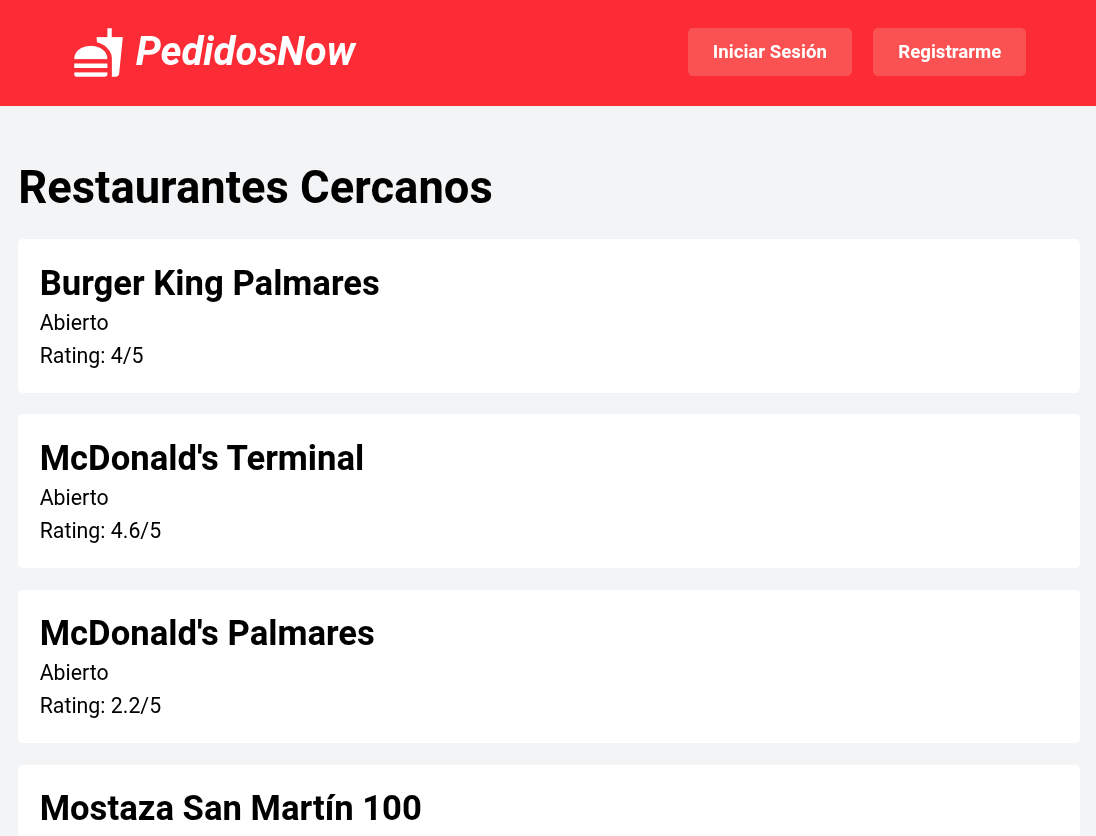
\includegraphics[width=10cm]{./img/public-locations.png}
    \caption{Pantalla de inicio.}
\end{figure}

Si hacemos click en una sucursal, podremos observar su menú, tal como lo muestra la siguiente figura. La pantalla indica el nombre de la sucursal, si está abierta o cerrada, su rating promedio, y los ítems de su menú. Para cada item se indica su nombre, categoría, descripción y precio. La funcionalidad del botón ``Comprar'' no está implementada.

\begin{figure}[H]
    \centering
    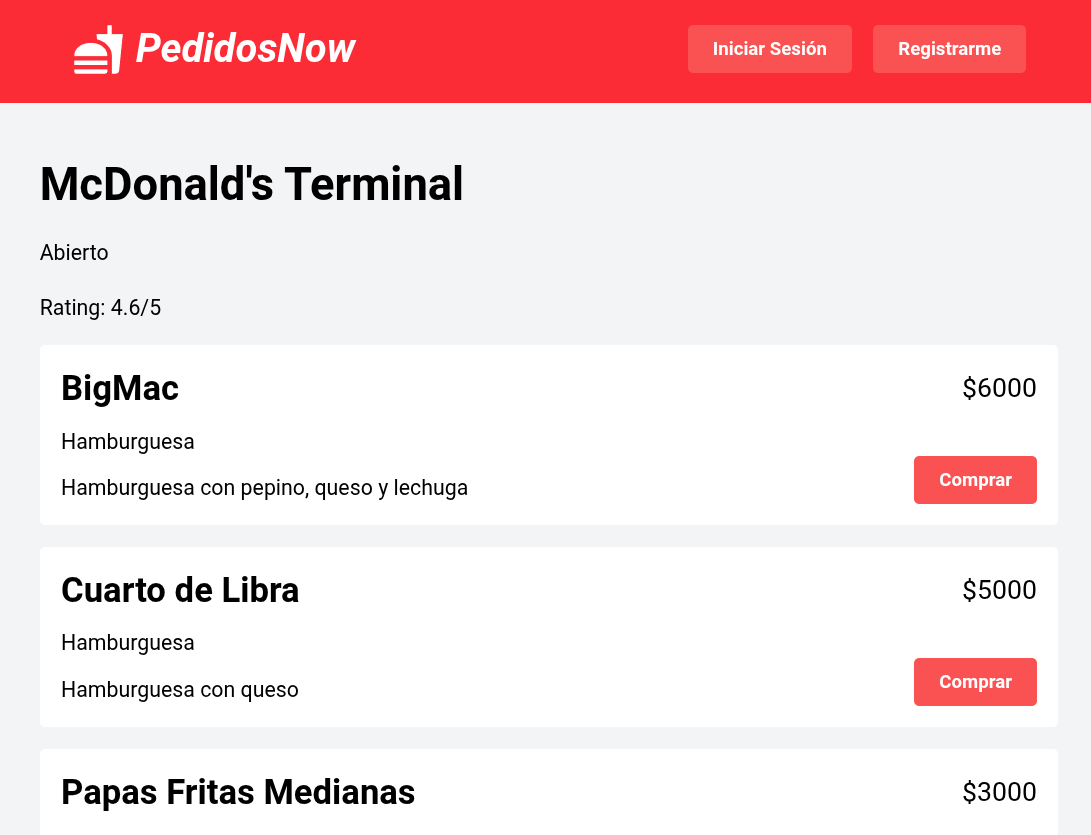
\includegraphics[width=10cm]{./img/public-items.png}
    \caption{Pantalla de menú de sucursal.}
\end{figure}

Para poder hacer modificaciones en los datos del sistema, debemos iniciar sesión o registrarnos. El sistema solo permitirá modificar aquellos recursos que sean del propio usuario, y no aquellos de otros usuarios. Para ello, hacemos click en el botón ``Iniciar Sesión'' o ``Registrarme'' en el encabezado de la página. Se abrirá una página como la de la siguiente figura.

\begin{figure}[H]
    \centering
    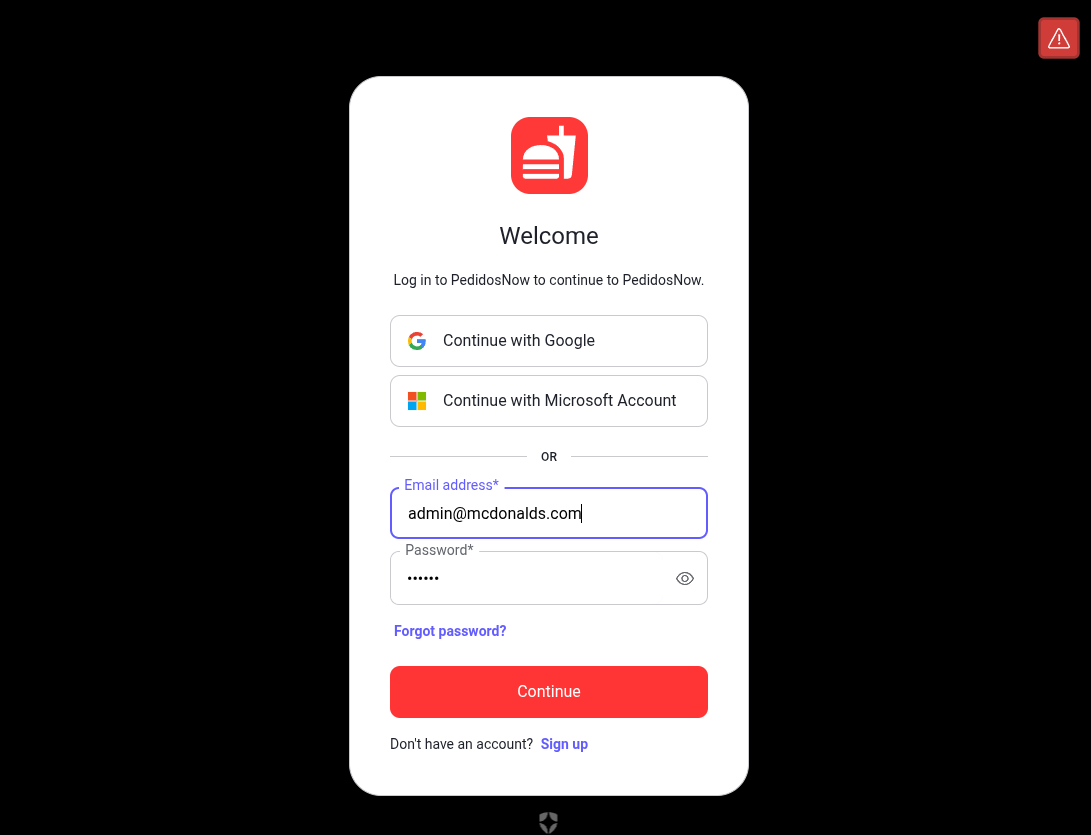
\includegraphics[width=10cm]{./img/login.png}
    \caption{Pantalla de inicio de sesión / registro.}
\end{figure}

En caso de crear un usuario nuevo, una vez autenticado, será redirigido a un formulario para completar su registro, como el de la siguiente figura, donde se deberá indicar el nombre de la cadena de restaurantes, y el domicilio legal.

\begin{figure}[H]
    \centering
    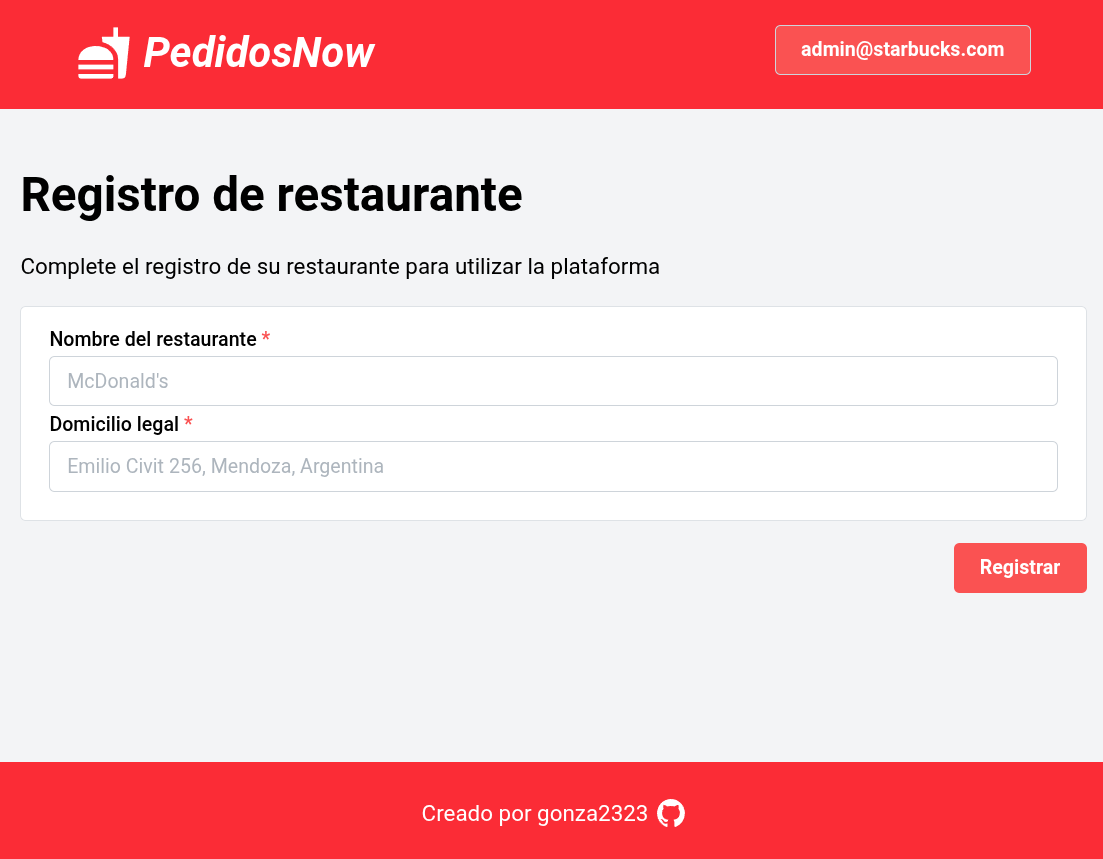
\includegraphics[width=10cm]{./img/login-form.png}
    \caption{Pantalla de registro de nuevo restaurante.}
\end{figure}

Una vez registrado y autenticado el usuario, se indicará el nombre del restaurante en el encabezado de la página, como se muestra en la siguiente figura. Si se hace click sobre el mismo, se abrirá un menú desplegable con opciones para ir a la página de administración de sucursales, y cerrar sesión.

\begin{figure}[H]
    \centering
    
\includegraphics[width=4cm]{./img/dropdown.png}
    \caption{Menú desplegable para usuarios autenticados.}
\end{figure}

Si el usuario hace click en ``Administrar Sucursales'', será redirigido a una página como la de la siguiente figura. En la misma, se indican las sucursales de su restaurante, sus nombres, rating promedio, y si están abiertas o cerradas. Para cada una de ellas, hay botones para abrir, cerrar, editar o borrar esa sucursal en particular. También hay botones para añadir una nueva sucursal, o generar un reporte de los ingresos generados por cada una.

\begin{figure}[H]
    \centering
    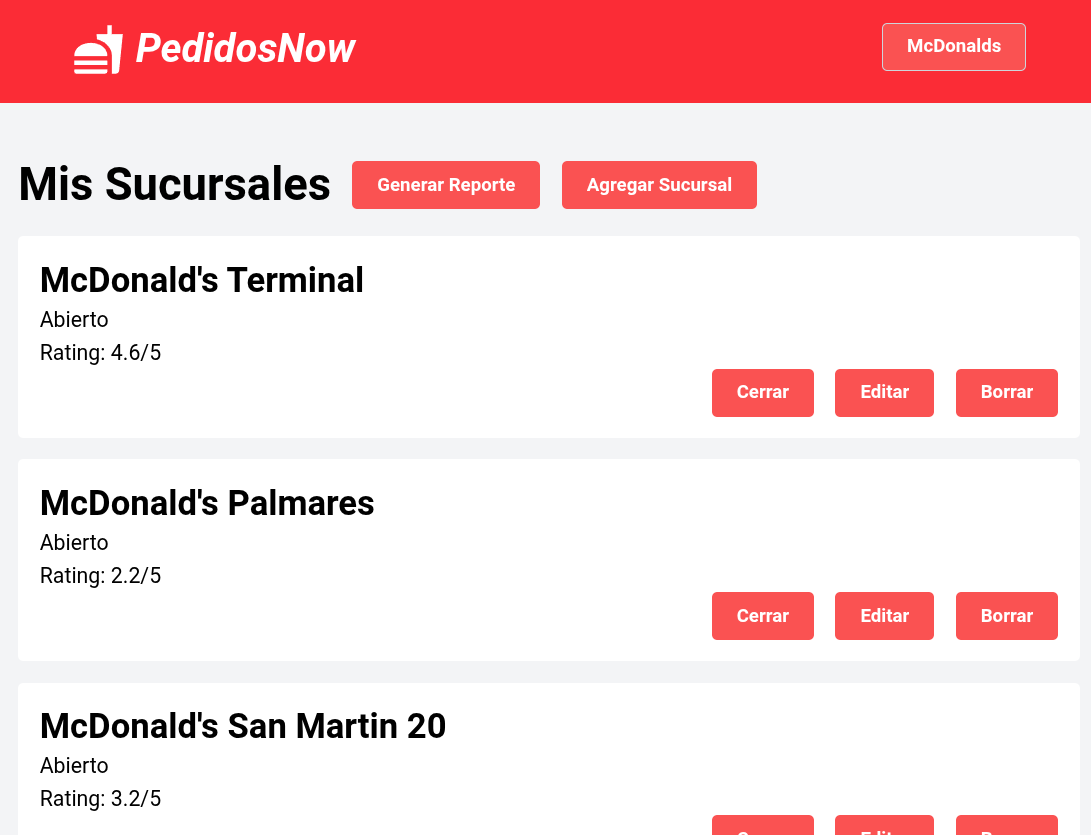
\includegraphics[width=10cm]{./img/locations.png}
    \caption{Página de gestión de sucursales.}
\end{figure}

Si el usuario hace click en ``Agregar Sucursal'', se abrirá un formulario como el de la siguiente figura. El usuario debe completar el nombre y los campos de dirección de la misma y presionar ``Agregar''.

\begin{figure}[H]
    \centering
    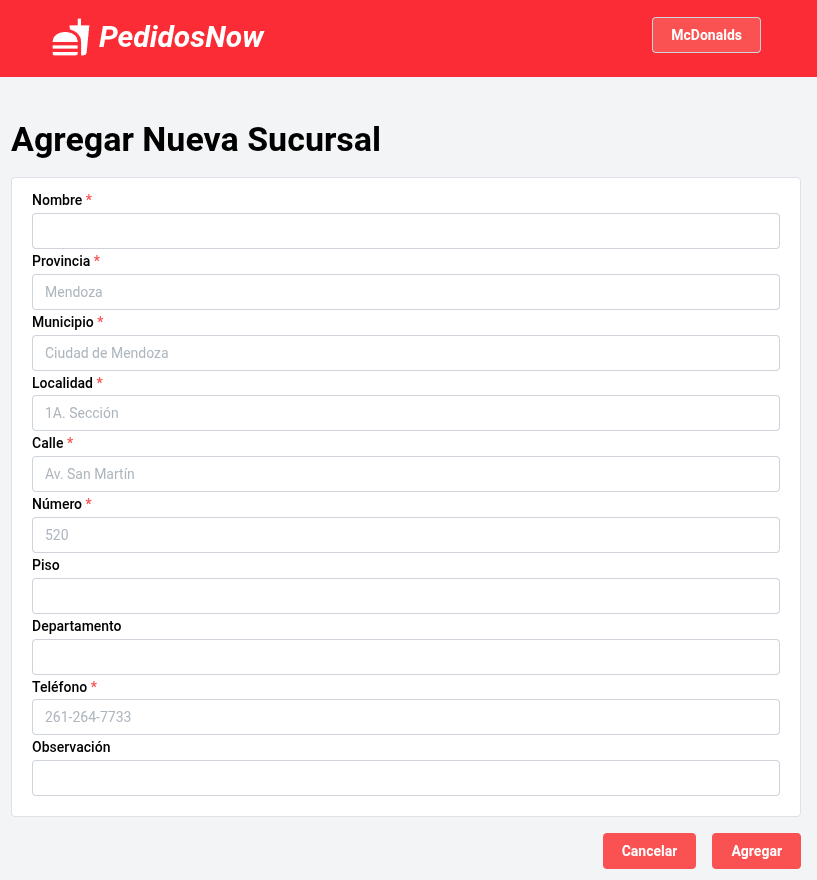
\includegraphics[width=10cm]{./img/locations-add.png}
    \caption{Formulario de alta de sucursal.}
\end{figure}

Si en la pantalla de gestión de sucursales, el usuario hace click en el botón ``Editar'' de alguna sucursal, será redirigido a un formulario para editar su nombre y dirección, como se muestra en la siguiente figura.

\begin{figure}[H]
    \centering
    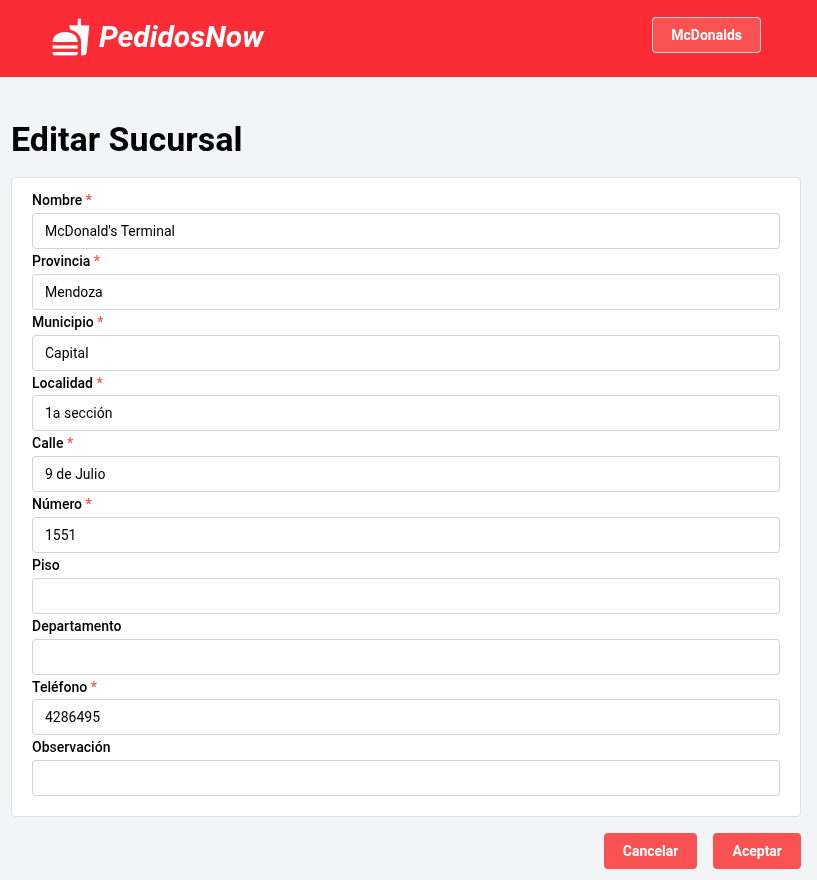
\includegraphics[width=10cm]{./img/location-edit.png}
    \caption{Formulario de modificación de sucursal.}
\end{figure}

Si en la pantalla de gestión de sucursales, el usuario hace click sobre alguna sucursal, será redirigido a la pantalla de gestión de menú de esa sucursal, donde podrá agregar, editar y modificar ítems del menú de la misma. Tal pantalla se muestra en la siguiente figura. En la misma se indican el nombre de la sucursal en cuestión, si está abierta o cerrada, su rating promedio, y los ítems de su menú. Para cada ítem, se indica su nombre, categoría, descripción, precio y disponibilidad. A su vez, cada ítem cuenta con botones para cambiar su disponibilidad, modificar sus datos y borrarlo. Al final de la página, encontramos un botón para agregar un nuevo ítem al menú.

\begin{figure}[H]
    \centering
    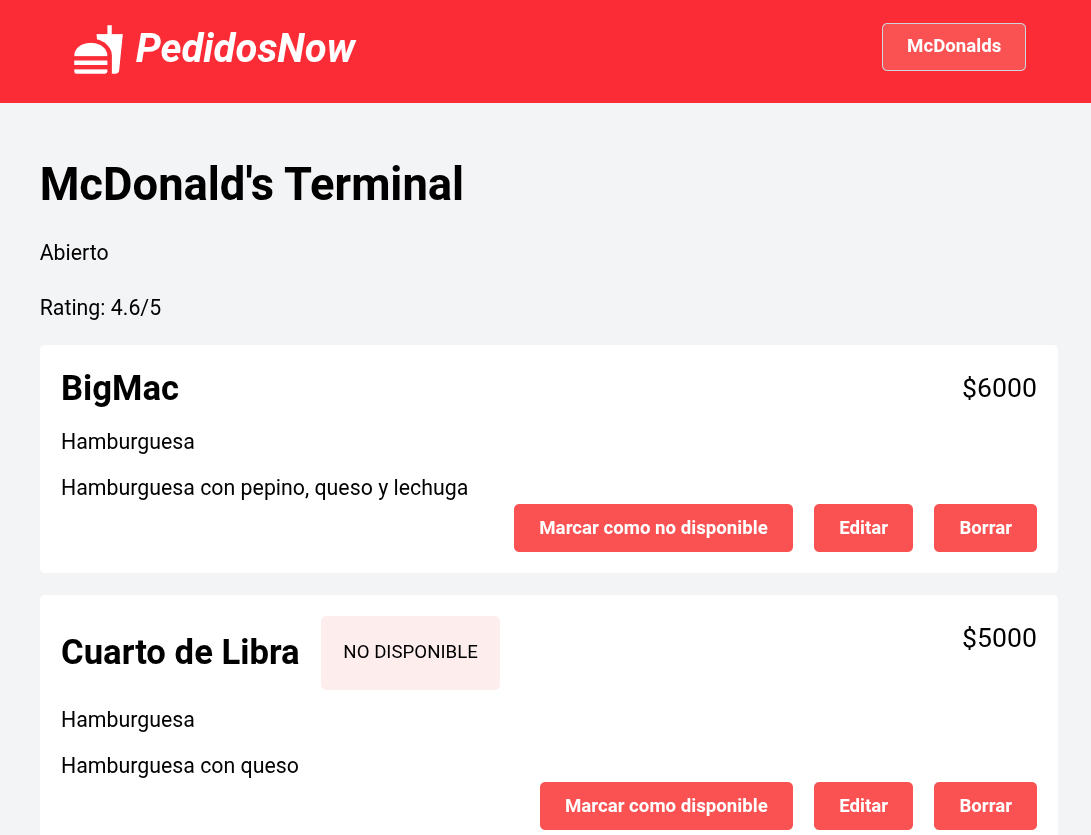
\includegraphics[width=10cm]{./img/items.png}
    \caption{Pantalla de gestión de menú de sucursal.}
\end{figure}

Si hacemos click en ``Agregar ítem al menú'', se abrirá un formulario como el de la siguiente figura. En el mismo, el usuario debe indicar el nombre, descripción, precio y categoría (de las cargadas ya en la base de datos), del ítem a agregar. Una vez listo, debe presionar ``Confirmar''.

\begin{figure}[H]
    \centering
    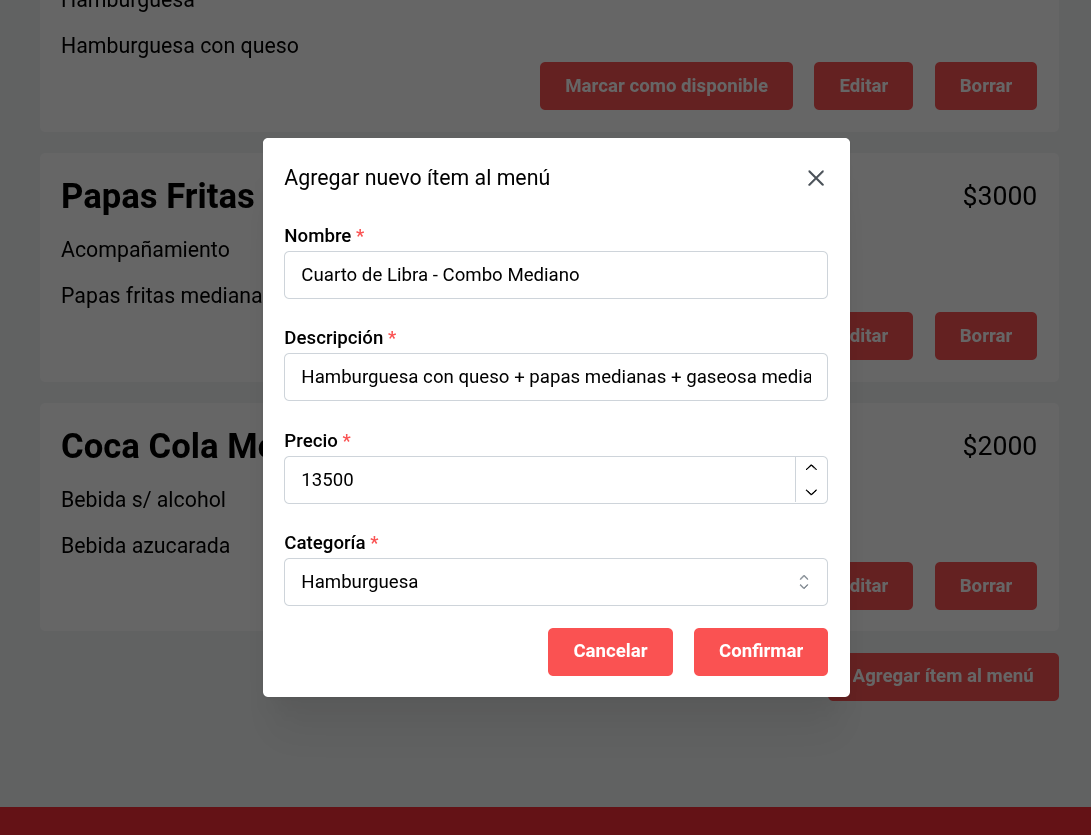
\includegraphics[width=10cm]{./img/item-add.png}
    \caption{Formulario de alta de ítem de menú.}
\end{figure}

Si hacemos click en el botón ``Editar'' de algún ítem del menú, se abrirá un formulario similar al anterior para modificar los datos del ítem en cuestión, tal como se muestra en la siguiente figura.

\begin{figure}[H]
    \centering
    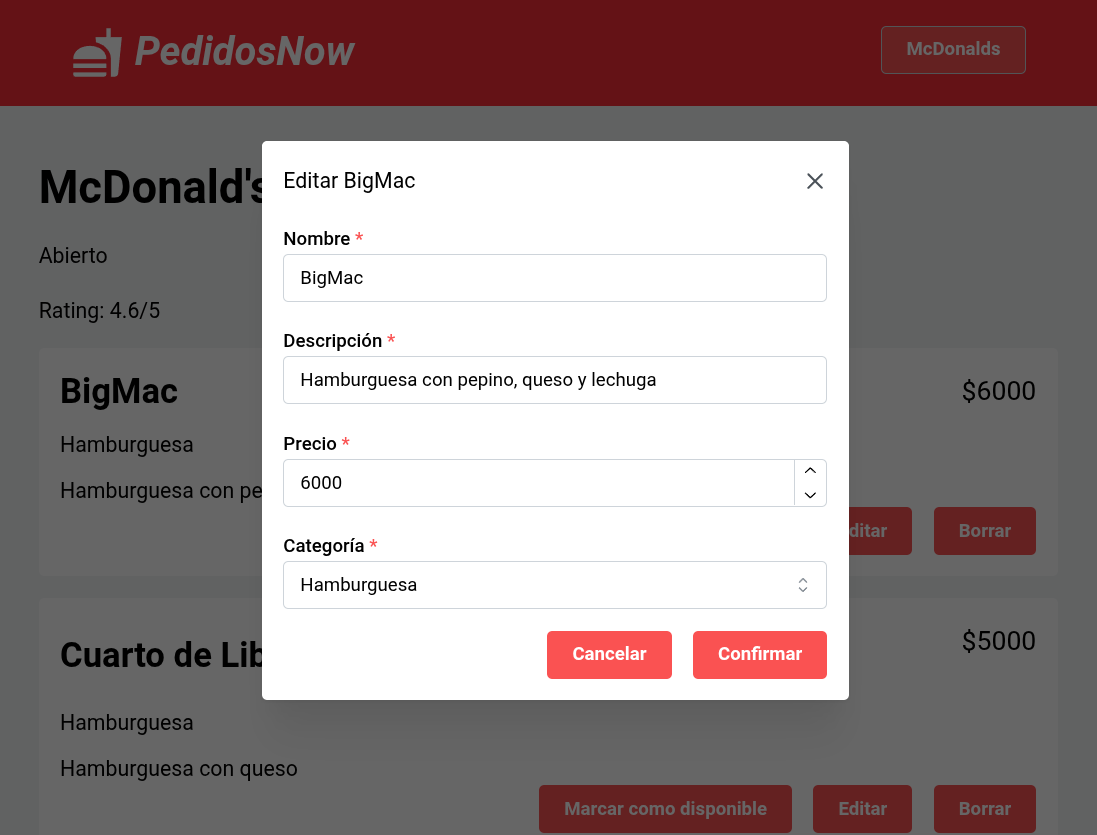
\includegraphics[width=10cm]{./img/item-edit.png}
    \caption{Formulario de modificación de ítem de menú.}
\end{figure}

Por otro lado, si en la pantalla de gestión de sucursales, hacemos click en el botón ``Generar Reporte'', se generará un reporte en formato PDF como el de la siguiente figura. El mismo contiene el nombre de la cadena de restaurantes, la dirección de mail asociada, y una tabla de las sucursales cargadas. Para cada sucursal, se indica si está actualmente abierta o cerrada, su rating promedio (si es que hay suficientes reseñas), la cantidad de pedidos que ha entregado, el monto promedio de los mismos, y la cantidad de ingresos totales que ha generado durante su existencia.

\begin{figure}[H]
    \centering
    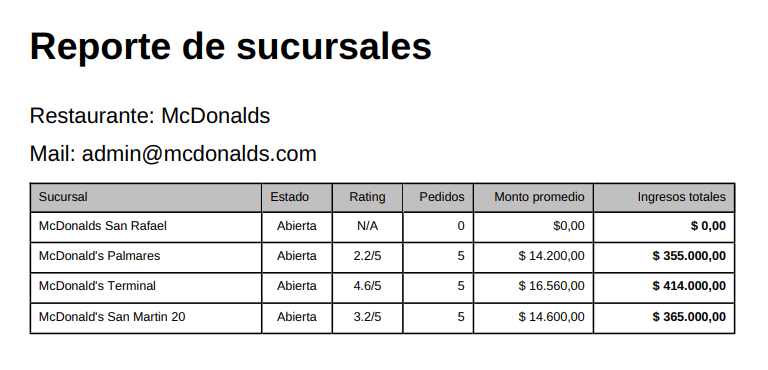
\includegraphics[width=10cm]{./img/report.png}
    \caption{Reporte de ingresos por sucursal.}
\end{figure}

Si en lugar de iniciar sesión como un restaurante, iniciamos sesión con una cuenta de administrador, el menú desplegable indicará ``Admin'', y ofrecerá la opción de ``Administrar Backups'', tal como se indica en la siguiente figura.

\begin{figure}[H]
    \centering
    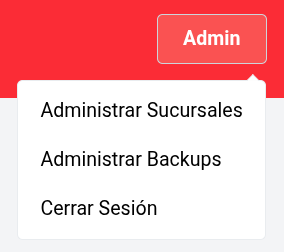
\includegraphics[width=4cm]{./img/admin-dropdown.png}
    \caption{Menú desplegable para administrador.}
\end{figure}

Si hacemos click en tal opción, se abrirá una pantalla como la de la siguiente figura. En la misma podemos ver una lista de los backups ya creados. Para cada uno, se indica su nombre, el cual incluye la hora y fecha de creación, y botones para descargar, eliminar o restaurar esa copia de seguridad. También hay botones para crear un nuevo backup y para subir un archivo de copia de seguridad.

\begin{figure}[H]
    \centering
    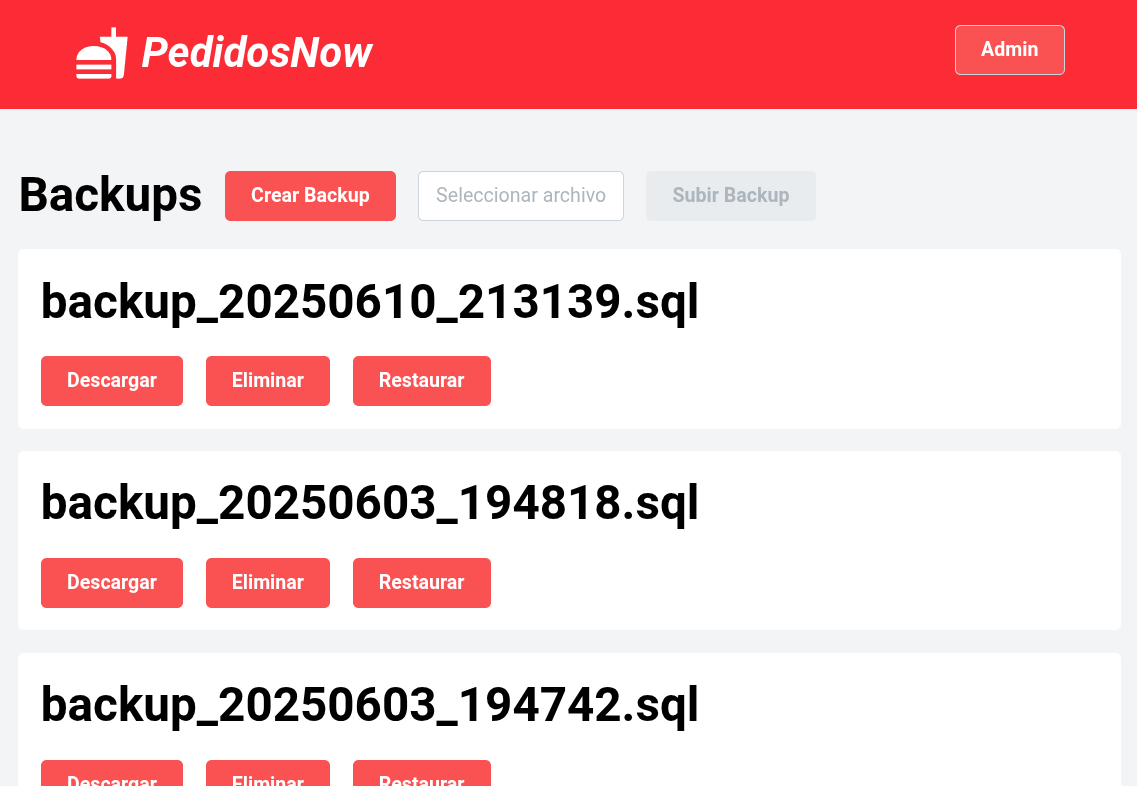
\includegraphics[width=10cm]{./img/admin-backups.png}
    \caption{Pantalla de gestión de copias de seguridad.}
\end{figure}



\section{Trabajos Futuros}

A continuación se detallan funciones que pueden implementarse en un futuro desarrollo del sistema, utilizando lo ya implementado en el modelo de datos.

\begin{enumerate}
    \item \textbf{Carrito de compras:} Permitir a los clientes añadir ítems del menú de una sucursal a su carrito de compras
    \item \textbf{Autenticación y registro para clientes y repartidores:} Agregar un sistema de roles para que puedan ingresar al sistema tanto clientes (para realizar órdenes) como repartidores (para aceptar pedidos y realizarlos). 
    \item \textbf{Filtrado de sucursales por distancia al cliente:} Utilizar la latitud y longitud de la dirección seleccionada del cliente y de las sucursales para solo mostrar aquellas sucursales dentro de determinado rango de distancia.
    \item \textbf{Sistema de asignación automática de repartidores:} El sistema debería elegir automáticamente al repartidor más apropiado para un envío en particular.
    \item \textbf{Sistema de pagos:} Una vez elegidos los productos, que el cliente pueda realizar el pago y que se encargue la orden a la sucursal seleccionada. También se debe realizar el pago al restaurante, y al repartidor.
    \item \textbf{Seguimiento en tiempo real:} Permitir a los clientes ver en tiempo real, a través de la interfaz gráfica, el estado de su pedido y la posición del repartidor en un mapa.
\end{enumerate}


\end{document}
